\documentclass[border=10pt]{standalone}

\usepackage{tikz}
\usepackage{tikzsymbols}
\usetikzlibrary{calc,patterns,shapes.geometric}

\def\centerarc[#1](#2)(#3:#4:#5){\draw[#1] ($(#2)+({#5*cos(#3)},{#5*sin(#3)})$) arc (#3:#4:#5);}

\begin{document}
	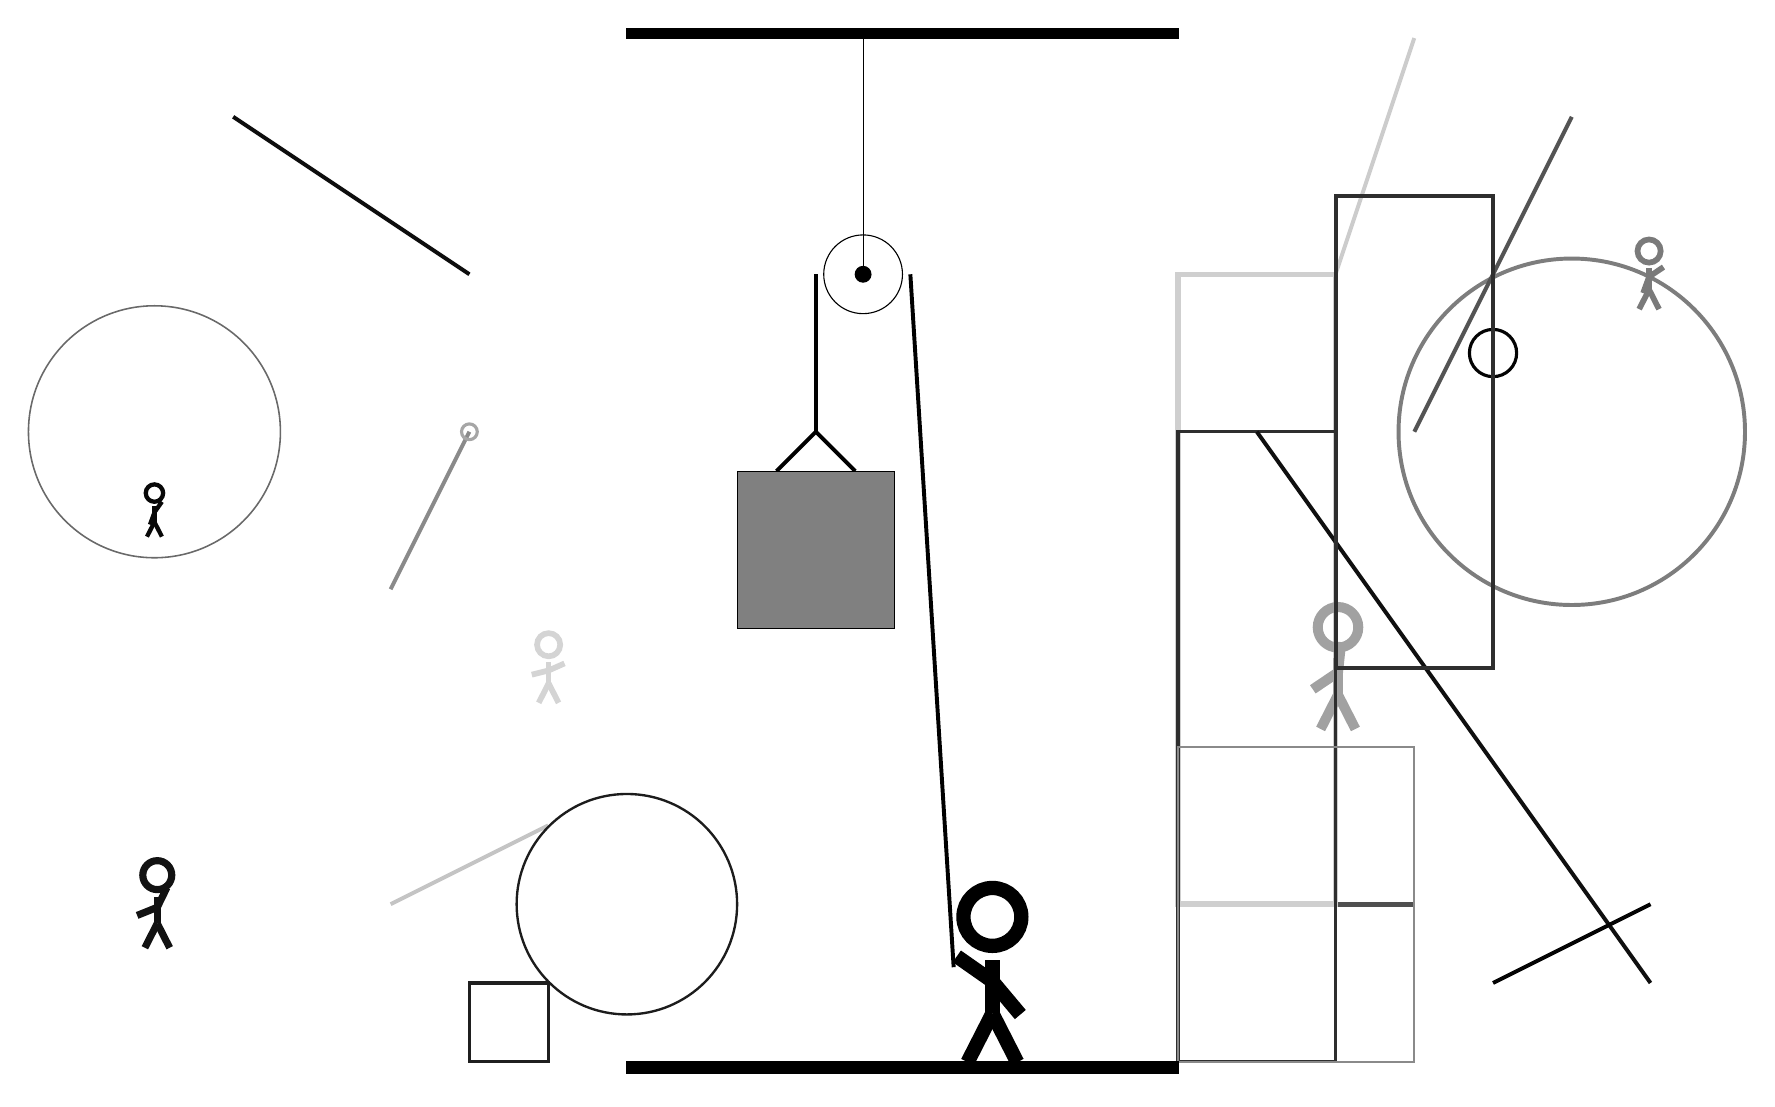
\begin{tikzpicture}
		%%%%% START %%%%%
		
		\draw[fill=black] (-2, 10) rectangle (5, 10.125);
		
		\draw (1, 7) circle (0.5);
		\draw[fill=black] (1, 7) circle (0.1);
		\draw (1, 10) -- (1, 7);
		
		\draw[line width=0.5mm] (-0.1, 4.5) -- (0.4, 5.0) -- (0.9, 4.5);
		\draw[fill=black!50] (-0.6, 4.5) rectangle (1.4, 2.5);
		
		\draw[line width=0.5mm] (0.4, 7) -- (0.4, 5.0);
		\centerarc[line width=0.5mm](1, 7)(0:180:0.6);
		\draw[line width=0.5mm](1.6, 7) -- (2.15, -1.8);
		
		\node at (2.6, -1.9) {\Strichmaxerl[10][-35][-50]};
		
		\draw[line width=0.5mm, color=black!46](-5, 3) -- (-4, 5);
		
		\node[line width=0.2mm, color=black!17] at (-3, 2) {\Strichmaxerl[4][14][24]};
		\draw[line width=0.6mm, color=black!69] (6, -1) rectangle (8, -1);
		\node[line width=0.2mm, color=black!97] at (-8, 4) {\Strichmaxerl[3][70][55]};
		\draw[line width=0.5mm, color=black!12] (7, 0) rectangle (7, 1);
		
		\draw[line width=0.7mm, color=black!19] (5, -1) rectangle (7, 7);
		
		\draw [line width=0.2mm, color=black!59](-8, 5) circle (1.6);
		
		\draw [line width=0.5mm, color=black!51](10, 5) circle (2.2);
		\draw[line width=0.4mm, color=black!88] (-3, -2) rectangle (-4, -3);
		\node[line width=0.2mm, color=black!37] at (7, 2) {\Strichmaxerl[7][34][84]};
		
		\draw[line width=0.5mm, color=black!23](-3, 0) -- (-5, -1);
		
		\draw [line width=0.4mm, color=black!35](-4, 5) circle (0.1);
		\draw [line width=0.4mm, color=black!99](9, 6) circle (0.3);
		
		\draw [line width=0.3mm, color=black!89](-2, -1) circle (1.4);
		\node[line width=0.5mm, color=black!52] at (11, 7) {\Strichmaxerl[4][70][34]};
		\draw[line width=0.5mm, color=black!20](7, 7) -- (8, 10);
		
		\draw[line width=0.4mm, color=black!82] (5, -3) rectangle (7, 5);
		\draw[line width=0.5mm, color=black!67](10, 9) -- (8, 5);
		\draw[line width=0.3mm, color=black!46] (5, 1) rectangle (8, -3);
		\draw[line width=0.5mm, color=black!94](6, 5) -- (11, -2);
		\node[line width=0.3mm, color=black!93] at (-8, -1) {\Strichmaxerl[5][22][64]};
		
		\draw[line width=0.5mm, color=black!95](-7, 9) -- (-4, 7);
		
		\draw[line width=0.5mm, color=black!82] (7, 2) rectangle (9, 8);
		\draw[line width=0.5mm, color=black!99](9, -2) -- (11, -1);
		
		\draw[fill=black] (-2, -3) rectangle (5, -3.15);
		
		%%%%% END %%%%%
	\end{tikzpicture}
\end{document}